\documentclass[aspectratio=169]{beamer}
\usepackage{graphicx} % Required for inserting images

%aspectratio: es la relación entre el ancho y el alto de la diapositiva
% relación 16:9
% relación 4:3 por default
% relación 16:10
% relación 14:9
% relación 5:4

\usetheme{PaloAlto} %formato de las diapositivas, con índice, título en la parte inferior, número de página, etc.
\usecolortheme{crane} %distribución de colores de las diapositivas y los bloques asociades a usetheme.

\title{Presentación con Beamer}
\author{Miguel Carrillo }
\date{5 de septiembre de 2024}

\begin{document}


\begin{frame}[plain]
\titlepage
\begin{center}
	
\includegraphics[scale=0.2]{imagenes/logo_unam.jpg}\hspace{8cm}
	
\includegraphics[scale=0.04]{imagenes/ciencias.png}  
%    
\includegraphics[scale=0.2]{logo_unam.jpg} \hspace{8cm}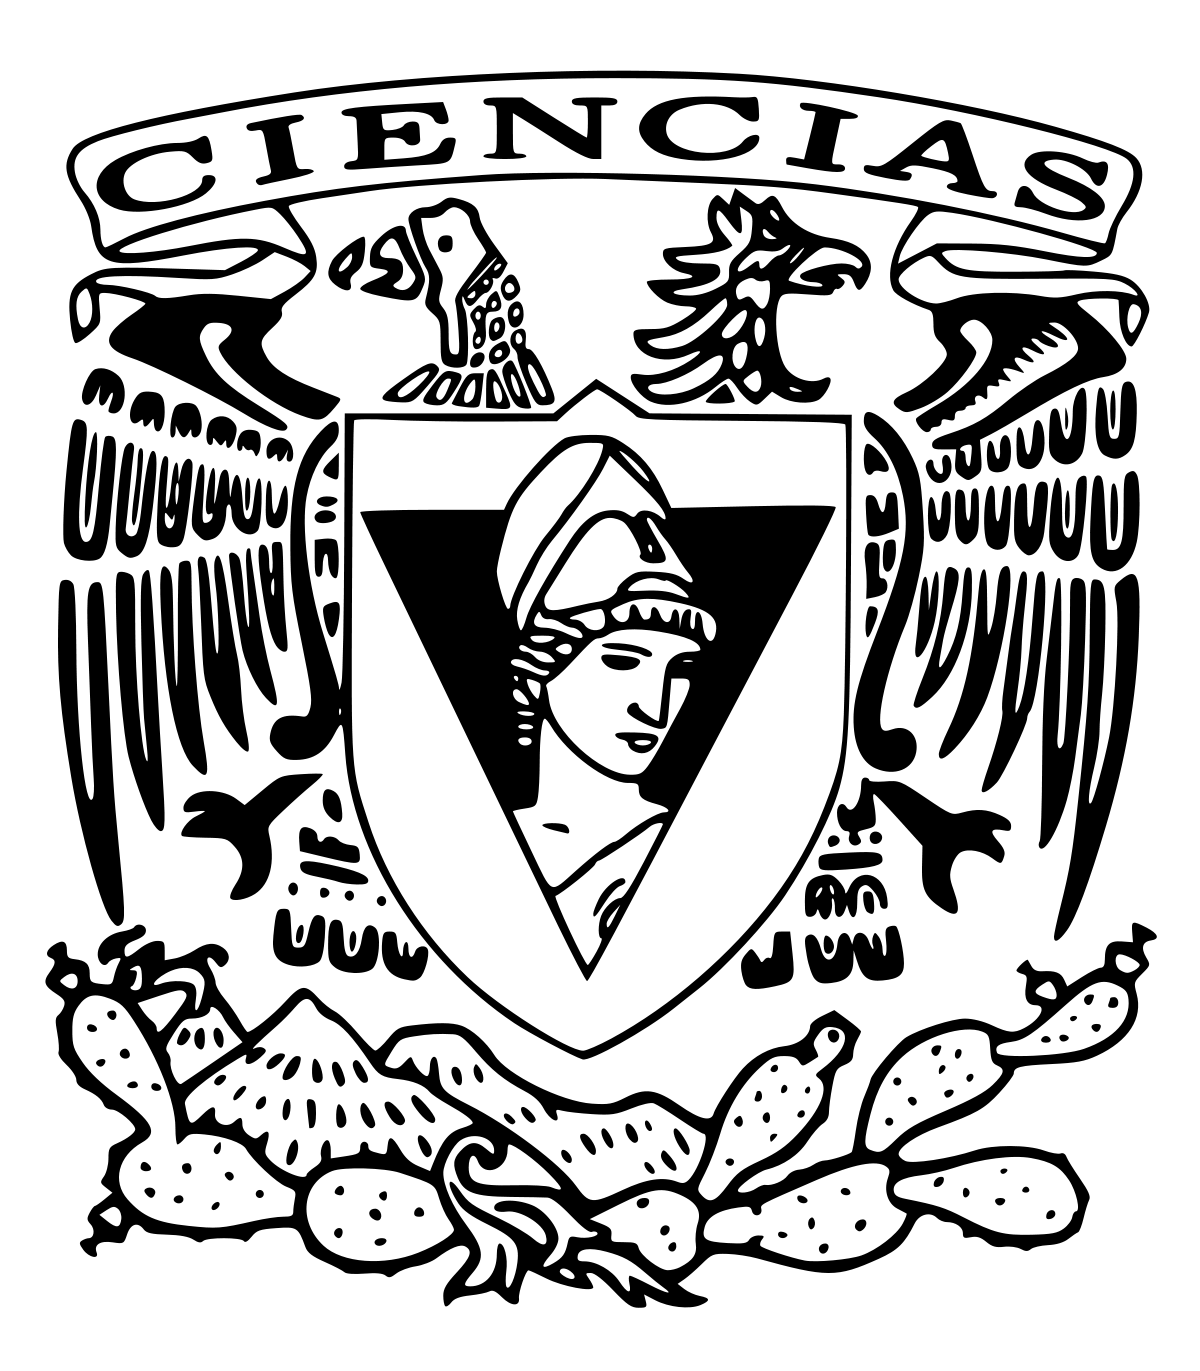
\includegraphics[scale=0.04]{escudo_fciencias.png}    
\end{center}

\end{frame}


\section{Introducción}
\begin{frame}{Primera diapositiva}
    Hola. Esta es mi primera diapositiva. Incluir primer bloque. \pause
% opciones de bloque son: block, exampleblock y alertblock

    \begin{block}{Bloque sencillo}  
        Este es el primer bloque. \pause
        \begin{enumerate}
            \item Bloque sencillo \pause
            \item Bloque ejemplo \pause
            \item Bloque alerta
        \end{enumerate}
    \end{block}
\end{frame}





\subsection{El juego del ajedrez}
\begin{frame}{Ajedrez}
    El ajedrez es un juego de mesa (o de tablero) entre dos oponentes. Se compone de 8 peones, dos caballos, las torres, los alfiles, la reina y el rey.

\begin{exampleblock}{Piezas del ajedrez}
Las piezas del ajedrez son: 
    \begin{itemize}
        \item Peones
        \item Alfiles
        \item Torres
    \end{itemize}
    \end{exampleblock}
\end{frame}


\begin{frame}{Bloque alerta}
    Por último, el bloque alerta.

    \begin{alertblock}{Último ejemplo}
        Bloque alerta
    \end{alertblock}
\end{frame}


\end{document}
